\documentclass[a4paper,12pt]{scrreprt}

\renewcommand*{\chapterpagestyle}{scrheadings}



%Inhalt der Titelseite
\newcommand{\Titel}{Webvisualisierung von Prozesskomponenten in der Bildgebenden Qualitätskontrolle}
\newcommand{\Art}{Studienarbeit 2}
\newcommand{\Vorname}{Andreas}
\newcommand{\Nachname}{Braig}
\newcommand{\Studiengang}{Elektrotechnik}
\newcommand{\Abgabedatum}{02.01.2025}
\newcommand{\Bearbeitungszeitraum}{07.01.2025 - 07.04.2025}
\newcommand{\Matrikelnummer}{6481829}
\newcommand{\Kurskrzl}{TEL22AT1}
\newcommand{\Abteilung}{PAPI-EAM}
\newcommand{\Ausbildungsfirma}{ABB AG}
%\newcommand{\BetrieblicherBetreuer}{Florian Diehm}
\newcommand{\BetreuerDHBW}{Prof. Dr.-Ing. Bozena Lamek-Creutz}

%Nur benötigt wenn Sperrvermerk verwendet wird
\newcommand{\SperrvermerkAuslaufDatum}{XX.XX.XXXX}

\newcommand{\ArtDerArbeit}{T3\_3200}

% Pakete laden
\usepackage[utf8]{inputenc}
\usepackage[T1]{fontenc}
\usepackage[ngerman]{babel}
\usepackage{helvet} % Arial Schriftart
\renewcommand{\familydefault}{\sfdefault} % Setzt die Standardschriftart auf sans-serif (Arial)
\usepackage[printonlyused]{acronym}
\usepackage[onehalfspacing]{setspace}
\usepackage[left=2.5cm,right=2.5cm,bottom=4cm,top=2.5cm]{geometry}
\usepackage{ragged2e}
\usepackage{listings}
\usepackage{graphicx}
\usepackage{subcaption}
\usepackage{tabularx}
\usepackage{tikz}
\usepackage[style=ieee]{biblatex}
\usepackage{lipsum} % Dummy Text
\usepackage{tabularray}
\usepackage[x11names]{xcolor} % Für erweiterte Farboptionen
\usepackage{pdfpages}
\usepackage{float}
\usepackage{caption}
\usepackage{csquotes}
\usepackage{enumitem}
\usepackage{amssymb}
\usepackage[toc,page]{appendix}
\usepackage{pifont}
\usepackage{colortbl}
\usepackage{booktabs}
\usepackage{courier}
\usepackage[gen]{eurosym}
\usepackage{xcolor} % Falls noch nicht enthalten
\usepackage{listings}

%für die Matrix
\usepackage{amsmath}
\usepackage{array}


\addbibresource{resources/directories/bibliography.bib}

% Automatisch eine Leerzeile nach einem Absatz einfügen
\setlength{\parskip}{\baselineskip}


% % Kopf- und Fußzeile
% \usepackage[headsepline=0.1pt, footsepline=0.1pt, automark]{scrlayer-scrpage}
% \pagestyle{scrheadings}
% \clearpairofpagestyles % Löscht voreingestellte Kopf- und Fußzeilen
% \ofoot[\pagemark]{\pagemark} % Seitenzahl mittig unten
% \ihead{\upshape\Vorname{} \Nachname{}} % Kopfzeile ohne Kursivschrift
% \ohead{\upshape\Art{}} % Kopfzeile ohne Kursivschrift

\usepackage[headsepline=0.1pt, footsepline=0.1pt, automark]{scrlayer-scrpage}
% Falls noch nicht enthalten, für Farben notwendig

\setkomafont{pageheadfoot}{\color{lightgray}} % Kopf- und Fußzeile grau einfärben

\pagestyle{scrheadings}
\clearpairofpagestyles % Löscht voreingestellte Kopf- und Fußzeilen

% Kopf- und Fußzeile grau einfärben
\ihead{\textcolor{lightgray}{\upshape\Vorname{} \Nachname{}}} % Kopfzeile ohne Kursivschrift
\ohead{\textcolor{lightgray}{\upshape\Art{}}} % Kopfzeile ohne Kursivschrift
\ofoot[\textcolor{lightgray}{\pagemark}]{\textcolor{lightgray}{\pagemark}} % Seitenzahl mittig unten in Grau

% Charter Schriftart für Kapitelüberschriften
%\setkomafont{disposition}{\normalfont\bfseries}

% Formatierung der Chapter-Überschriften
\makeatletter
\renewcommand\@makechapterhead[1]{%
	\vspace*{0\p@}%
	{\parindent \z@ \raggedright
		\normalfont
		\interlinepenalty\@M
		\fontsize{16pt}{16pt}\selectfont \bfseries \thechapter.\  #1\par\nobreak
		\vskip 10\p@
}}
\renewcommand\section{\@startsection {section}{1}{\z@}%
	{-2.5ex \@plus -1ex \@minus -.2ex}% Abstand vor der Überschrift
	{2.3ex \@plus.2ex}% Abstand nach der Überschrift
	{\normalfont\fontsize{14pt}{14pt}\selectfont\bfseries}}
\renewcommand\subsection{\@startsection {subsection}{2}{\z@}%
	{-1.25ex\@plus -1ex \@minus -.2ex}% Abstand vor der Überschrift
	{1.5ex \@plus .2ex}% Abstand nach der Überschrift
	{\normalfont\fontsize{12pt}{12pt}\selectfont\bfseries}}
\makeatother





% Abstand vor und nach Kapitelüberschriften
\renewcommand*{\chapterheadstartvskip}{\vspace*{1cm}}
\renewcommand*{\chapterheadendvskip}{\vspace{2\baselineskip}}

% Grafikpfad definieren
\graphicspath{{resources/images/}}

\setlength{\parindent}{0pt}

% Für Zitierung von URLs
\newcommand*{\quelle}{% 
	\footnotesize Quelle: 
}
\urlstyle{same}

\newcommand{\code}[1]{\texttt{#1}}


\definecolor{XMLgreen}{HTML}{697821}

\lstdefinelanguage{Python}{
	morekeywords={class, def, val, return, if, else, for, while, in, throw, try, catch,import},
	sensitive=true,
	comment=[l][\%],
	morecomment=[s][/*][*/],
	morestring=[b]"
}

\lstdefinelanguage{json}{
	morekeywords={true, false, null},
	sensitive=false,
	comment=[l][//],
	morestring=[b]",
}

% Listings-Style für JSON anpassen
\lstdefinestyle{json}{
	language=json,
	basicstyle=\ttfamily\scriptsize,
	numbers=left,
	numberstyle=\tiny\color{gray},
	breaklines=true,
	captionpos=b,
	frame=single,
	stringstyle=\color{blue},
	keywordstyle=\color{red}\bfseries, % Schlüsselwörter in Rot und fett
	commentstyle=\color{gray}, % Kommentare in Grau
	showstringspaces=false,
	stringstyle=\color{orange},
	tabsize=4
}

% Listings-Style für Python anpassen
\lstdefinestyle{python}{
	language=Python,
	basicstyle=\ttfamily\scriptsize,
	numbers=left,
	numberstyle=\tiny\color{gray},
	breaklines=true,
	captionpos=b,
	frame=single,
	keywordstyle=\color{blue}\bfseries,
	commentstyle=\color{green},
	stringstyle=\color{orange},
	showstringspaces=false,
	tabsize=4,
	morekeywords={self, None, True, False} % Weitere Schlüsselwörter hinzufügen
}

% Definiere die benutzerdefinierte Umgebung für Code
\newenvironment{mycode}
{\captionsetup{type=listing}} % Setzt den Typ der Beschriftung auf "listing"
{} % Ende der Umgebung (kann leer bleiben)


%Für Links und Hyperlinks
\usepackage[colorlinks = true,
linkcolor = black,
urlcolor  = black,
citecolor = black]{hyperref}

%Eigenschaften des PDF Dokuments anpassen (Titel, Art der Arbeit, Autor)
\hypersetup{pdftitle={\Titel},
	pdfsubject={\Art},
	pdfauthor={{\Vorname} {\Nachname}}
}




\begin{document}
	
	\pagestyle{empty}

%===========Logos============================================
%DHBW_Logo
\begin{tikzpicture}[remember picture,overlay]
	\node[anchor=north east,inner xsep=2.5cm, inner ysep=1.5cm] at (current page.north east)
	{
\includegraphics[scale=0.25]{dhbw-logo.png}};
\end{tikzpicture}

%Firmen Logo
\begin{tikzpicture}[remember picture,overlay]
	\node[anchor=north west,inner xsep=2.5cm, inner ysep=2cm] at (current page.north west)
	{
\includegraphics[scale=1]{ABB_Logo.png}};
\end{tikzpicture}

%===========Inhalt===========================================
\vspace{2cm}

\begin{center}
	\LARGE{\textbf{\Titel}} \\
	\vspace{0.5cm}
	\large{\textbf{\Art}}
\end{center}

\vspace{1cm}

\begin{center}
	des Studienganges \Studiengang \\
	an der Dualen Hochschule Baden-Württemberg Mannheim
\end{center}

\vspace{0.75cm}

\begin{center}
	von \\
	\Vorname{} \Nachname
\end{center}

\vspace{0.75cm}

\begin{center}
	\Abgabedatum
\end{center}

\vspace{1.5cm}

\begin{tabularx}{\textwidth}{l@{\hspace{2cm}}X}
	Bearbeitungszeitraum:            & \Bearbeitungszeitraum        \\
	Matrikelnummer, Kurs:            & \Matrikelnummer, \Kurskrzl   \\
	Ausbildungsfirma:                & \Ausbildungsfirma            \\
	Abteilung:                       & \Abteilung\\
	Betreuer der Dualen Hochschule:  & \BetreuerDHBW                \\
	& \\ & \\
\end{tabularx}


	
	\pagenumbering{Roman}
	
	\chapter*{Erklärung}

Ich versichere hiermit, dass ich die vorliegende Arbeit mit dem Thema: \glqq \Titel{}\grqq{} selbstständig verfasst und keine anderen als die angegebenen Quellen und Hilfsmittel benutzt habe. 
Ich versichere zudem, dass die eingereichte elektronische Fassung mit der gedruckten Fassung übereinstimmt.
\\
\\

\noindent
\begin{tabularx}{\textwidth}{@{\hspace{0pt}}p{5cm} X p{5cm}@{\hspace{0pt}}} \cline{1-1} \cline{3-3}
	Ort, Datum &  & Unterschrift 
\end{tabularx}

	\chapter*{Vorwort}
Diese Studienarbeit beschäftigt sich mit der Entwicklung und Umstrukturierung eines intelligenten Pflanzenbewässerungssystems, das über ein App-Interface gesteuert wird. Sie wurde im Rahmen der fünften Theoriephase an der \ac{dhbw} im Zeitraum vom 30.09.2024 bis zum 02.01.2025 angefertigt. Da das Projekt in zwei Teile untergliedert ist, wird im Verlauf dieser Arbeit gegebenenfalls auf den zweiten Bericht verwiesen, wobei einige inhaltliche Überschneidungen möglich sind.

Der erste Teil des Projekts trägt den Titel ``Design und Entwicklung eines smarten Bewässerungssystems für Pflanzen'' und beschäftigt sich mit den Hardwarekomponenten, den durchgeführten Messungen sowie deren Umsetzung. Der vorliegende Teil widmet sich dem App-Interface und der Schnittstelle zum verwendeten Mikrocontroller.

An dieser Stelle möchte ich mich herzlich bei meiner Kommilitonin Hannah Grüne sowie bei meiner Betreuerin \BetreuerDHBW\ für ihre wertvolle Unterstützung bedanken.

	\chapter*{Zusammenfassung}



\chapter*{Abstract}


	
	% Inhaltsverzeichnis
	\addcontentsline{toc}{chapter}{Inhaltsverzeichnis}\tableofcontents\clearpage
	
	% Abbildungsverzeichnis
	\addcontentsline{toc}{chapter}{Abbildungsverzeichnis}\listoffigures\clearpage
	
	% Listingverzeichnis
	\addcontentsline{toc}{chapter}{Listingverzeichnis}\lstlistoflistings\clearpage
	
	% Abkürzungsverzeichnis
	\chapter*{Abkürzungsverzeichnis}
\begin{acronym}[SBC]                
	\acro{CNN}{Convolutional Neural Network}
	\acro{API}{Application Programming Interface}
	\acro{api}[API]{Application Programming Interface}
	\acro{http}[HTTP]{Hypertext Transfer Protocol}
	\acro{rtc}[RTC]{Real Time Clock}
	\acro{ki}[KI]{Künstliche Intelligenz}
	\acro{dhbw}[DHBW]{Duale Hochschule Baden-Württemberg}
	\acro{PCB}[PCB]{Printed Circuit Board}
	\acro{cp}[CP]{Cyber-Physical}
	\acro{lab}[Lab]{Labor}
	\acro{cp-lab}[CP-Lab]{Cyber-Physical Lab}
	\acro{ABB}{Asea Brown Boveri}
	\acro{FESTO}{Festo Didactic SE}
	\acro{JSON}{JavaScript Object Notation}
	\acro{REST}{Representational State Transfer}
	\acro{HTTP}{Hypertext Transfer Protocol}
	\acro{URL}{Uniform Resource Locator}
	\acro{HTML}{Hypertext Markup Language}
	\acro{WSGI}{Web Server Gateway Interface}
	\acro{MVC}{Model-View-Controller}
	\acro{PC}{Personal Computer}
	\acro{USB}{Universal Serial Bus}
	\acro{SPS}{Speicherprogrammierbare Steuerung}
\end{acronym}


	
	\pagestyle{scrheadings}
	\pagenumbering{arabic}
	
	\chapter{Problemstellung und Ziel dieser Arbeit} \label{chap:problemstellung_und_ziel_dieser_arbeit}

Die zunehmende Automatisierung industrieller Prozesse erfordert zuverlässige Qualitätskontrollsysteme, insbesondere in der Fertigung von elektronischen Baugruppen wie Printed Circuit Boards \acp{PCB}. Im letzten Semester wurde ein KI-basiertes System entwickelt, das mittels TensorFlow Convolutional Neural Networks \acp{CNN} 
Defekte auf \acp{PCB} erkennt. Dieses System basiert auf einer Online-Implementierung ohne lokale Anpassungsmöglichkeiten und Benutzeroberfläche. 

Aktuell bestehen drei zentrale Herausforderungen: Erstens bietet die Online- Implementierung keine lokale Kontrolle über Parameter oder Daten, was die Flexibilität in industriellen Umgebungen limitiert. Zweitens fehlt eine intuitive Schnittstelle zur Visualisierung von 
Klassifizierungsergebnissen oder Anpassung von Einstellungen, was die Benutzerinteraktion erschwert. Drittens soll die Leistung der bisher verwendeten \ac{CNN}-Architektur evaluiert werden und weitere Architekturen oder Optimierungstechniken sollen getestet werden, um die
Erkennungsgenauigkeit zu verbessern.  

Ziel dieser Arbeit ist es, die bestehende Lösung in eine lokale Anwendung zu überführen, die folgende Kernkomponenten integriert: Eine zentrale Parametrisierung via JSON ermöglicht die flexible Steuerung aller Modell- und Systemparameter, während eine 
modularisierte Codebasis die Wartbarkeit und Wiederverwendbarkeit des Python-Codes verbessert. Zusätzlich soll eine Webanwendung mit Python-application Programming Interface \ac{API} entwickelt werden, die eine Echtzeit-Darstellung von \acp{PCB}-Bildern, Klassifizierungsergebnissen und Systemstatus bietet. 
Parallel erfolgt eine systematische Modellre-Evaluation, bei der das aktuelle \ac{CNN} mit alternativen Architekturen oder Optimierungstechniken verglichen wird.

Durch diese Maßnahmen soll die Darstellung der industriellen Anwendbarkeit im FESTO CP Lab gestärkt werden. Die neue Webvisualisierung soll greifbar machen, was bildverarbeitende Qualitätskontrolle bedeutet, indem sie die Echtzeit-Analyse und -Ergebnisse der \acp{PCB}-Bilder anschaulich darstellt. Benutzer können direkt sehen, dass Defekte erkannt und klassifiziert werden, was die Transparenz und Nachvollziehbarkeit des gesamten Prozesses erhöht.
	\chapter{Theoretische Grundlagen} \label{chap:theoretische_grundlagen}  % Theorie
	\chapter{Softwarekonzept} \label{chap:softwarekonzept}

\section{Architektur} \label{sec:architektur}

\section{Die Weboberfläche mittels Python Web API} \label{sec:weboberflaeche}
	\chapter{Implementierung} \label{chap:implementierung}

Nachdem im letzten Kapitel (siehe \autoref{chap:Konzept}) das Konzept der Lösung der Aufgabenstellung beschrieben wurde, wird in diesem Kapitel die Implementierung der Software beschrieben.
Ziel ist es, alle beschriebenen Aufgabenteile in Python umzusetzen und eine Software zu entwickeln, die in der Lage ist, die Anforderungen der Aufgabenstellung zu erfüllen. Ausschnitte aus dieser Software sind im Kapitel des Konzepts bereits beschrieben und werden hier weiter ausgeführt.

Die Implementierung erfolgt in mehreren Schritten:

\begin{enumerate}
    \item \textbf{Umzug auf lokale Programmierung} 
    \item \textbf{Einpflegen der JSON-Parameter} 
    \item \textbf{Entwicklung der API} 
    \item \textbf{Installation im Labor}

\end{enumerate}

In den folgenden Kapiteln werden die einzelnen Schritte genauer beschrieben.

\section{Umzug auf lokale Programmierung} \label{subsec:umzug_auf_lokale_programmierung}

Die Struktur dieser Implementierung folgt der Konzeption der Programmstruktur nach dem MVC-Prinzip \autoref{fig:MVC_struktur}, welches in \autoref{sec:architektur} beschrieben ist.
Dieses Modell trennt die Datenverarbeitung, die Darstellung und die Steuerung der Software in drei verschiedene Module auf.
Die Datenverarbeitung wird in einem eigenen Modul abgetrennt, Darstellung und Steuerung sind in der API zusammengefasst.

Das Pycore-Modul, welches diese benötigten, selbst entwickelten Bibliotheken zur Verfügung stellt, ist auch in \autoref{fig:Projektstruktur} als eigener Ordner mit Python-Skripten in seinen Unterverzeichnissen dargestellt. Es beinhaltet die Funktionen, welche den Datensatz aufbereiten und dem neuronalen Netzwerk zum Training zur Verfügung stellen.
Die wichtigsten Bestandteile sind die Konvertierung in Graustufen, die Aufteilung des Datensatzes in Trainings- und Testdaten sowie der Download des untrainierten neuronalen Netzwerks und dessen Parametrisierung bezüglich der Klassifikationsaufgabe.

\begin{figure}[H]
    \centering
    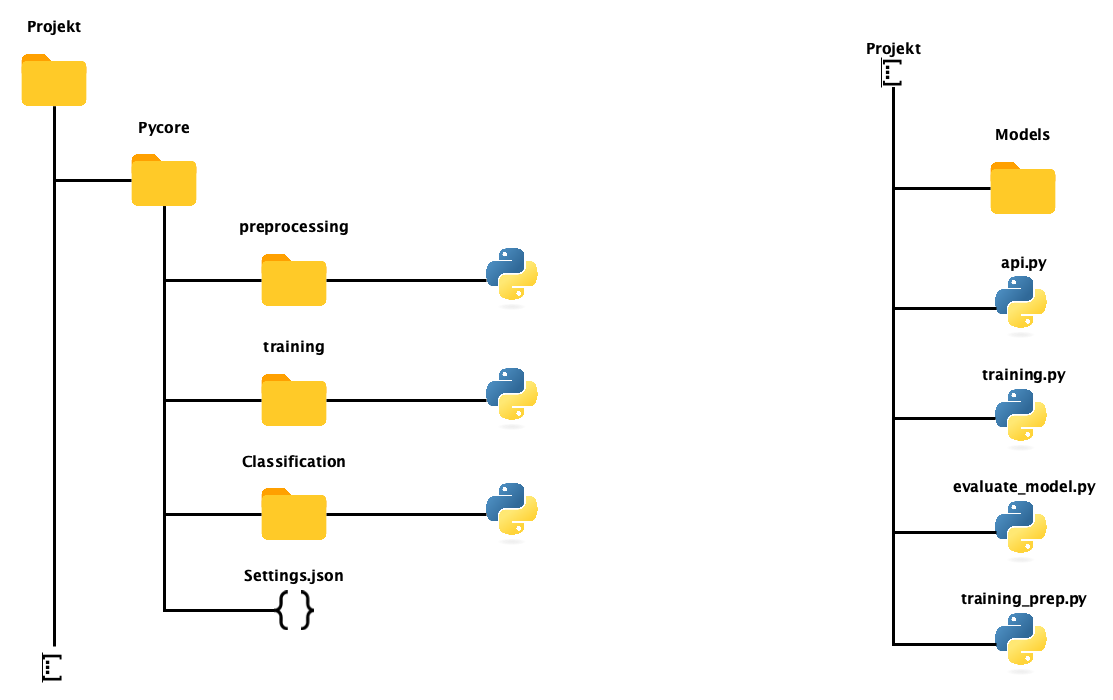
\includegraphics[width=0.8\textwidth]{Projektstruktur.png}
    \caption{Projektstruktur der Software im Dateiverzeichnis}
    \label{fig:Projektstruktur}
\end{figure}

Die in der Grafik \autoref{fig:Projektstruktur} dargestellte Dateistruktur repräsentiert ebenso die Struktur der Software. Die Funktionen werden in Bibliotheken im Pycore-Verzeichnis zusammengefasst. 
Sämtliche Daten werden in einem ausgegliederten Verzeichnis innerhalb des Projektverzeichnisses abgelegt. 

Im Projekthauptverzeichnis gibt es, neben des Pycore-Moduls und der Verzeichnisse für Trainings- und Testdaten, vier Python-Skripte. Diese können ausgeführt werden, um einzelne Teile der Software auszuführen.
\texttt{api.py} wird ausgeführt, um die Weboberfläche zu starten.
\texttt{train.py} wird ausgeführt, um das Modell zu trainieren.
\texttt{evaluate\_model.py} wird ausgeführt, um das Modell zu evaluieren und die in \autoref{sec:confusionmatrix} beschriebenen Werte zu erhalten. 
\texttt{training\_prep.py} kann ausgeführt werden, um den Datensatz zu verarbeiten, ohne das Modell zu trainieren.

Diese Skripte laden den jeweils benötigten Programmteil und die benötigten Parameter aus dem Pycore-Verzeichnis, führen die entsprechenden Funktionen aus und legen die Ergebnisse im Dateisystem ab.
Keines dieser Skripte ist über die Webanwendung zu erreichen, da sie nur für die interne Verwendung gedacht sind.

\section{Einpflegen der JSON-Parameter} \label{subsec:json_parameter}

Die Umsetzung des Konzeptes der Konfiguration der Programmparameter (siehe \autoref{sec:konfiguration}) erfolgt in Python mittels einer \ac{JSON}-Datei.
Diese Datei enthält alle Parameter, die für die Software benötigt werden.

\begin{lstlisting}[style=json, label=lst:json_example, caption={Beispiel einer \ac{JSON}-Datei mit Parametern des mobilnet Modells}]
    {
        "filepaths": {
            "good": "Bilder/Good_Pictures",
            "bad": "Bilder/Bad_Pictures",
            "good_gray": "Bilder/Good_Grayscale",
            "bad_gray": "Bilder/Bad_Grayscale",
            "train": "Bilder/train",
            "test":"Bilder/test",
            "validate":"Bilder/validate",
            "new": "Bilder/new"
        }
    }
\end{lstlisting}

Die Struktur der \ac{JSON}-Datei ist in \autoref{lst:json_example} dargestellt und wird in Python mittels des \texttt{json} Moduls eingelesen. Der hier dargestellte Ausschnitt beinhaltet alle wichtigen Dateipfade, um dem Python-Programm Zugriff zu den Trainings- und Testdaten sowie dem überwachten Ordner für neue Bilder zu gewähren. Er dient beispielhaft für das gesamte Programm. Ein Beispiel für das Einlesen der Datei ist in \autoref{lst:json_read} dargestellt.

\begin{lstlisting}[style=python, label=lst:json_read, caption={Einlesen der \ac{JSON}-Datei}]
    import json

    config_path = "pycore/setings.json"
    cf = json.load(open(config_path, 'r'))

    # Uebergabe der Parameter an die Funktionen
    uic.folder_to_grayscale(cf["filepaths"]["good"],cf["filepaths"]["good_gray"])
    uic.folder_to_grayscale(cf["filepaths"]["bad"],cf["filepaths"]["bad_gray"])

\end{lstlisting}

In diesem Codeausschnitt wird der Pfad zur Konfigurationsdatei festgelegt (Zeile 3) und die Datei wird eingelesen (Zeile 4). Die Parameter werden dann an die erste Funktion übergeben, welche die Bilder in Graustufen umwandelt und in einem separaten Verzeichnis ablegt (Zielverzeichnis siehe \autoref{lst:json_read}). Die Syntax für das Anwählen des Parameters ist \texttt{cf["filepaths"]["good"]}, wobei \texttt{cf} die Variable ist, in der die \ac{JSON}-Datei eingelesen wurde. Die \ac{JSON}-Datei wird als Array eingelesen, wobei der Zugriff auf die einzelnen Parameter über den Schlüssel in Textform erfolgt. In diesem Fall wird der Pfad zum Ordner mit den guten Bildern über den Schlüssel \texttt{"good"} angesprochen, während \texttt{"filepaths"} den Zugriff auf die passende Sektion des Arrays ermöglicht.

Angenommen der Benutzer wünscht ein anderes Verzeichnis für die Bilder, so kann er dies in der \ac{JSON}-Datei ändern und die Software erneut ausführen, ohne zu wissen, wo die Funktion, welche den Datensatz generiert, abliegt. 
Der gesamte Code dieses Projekts wurde nach diesem Schema aufgebaut, um eine einfache und einheitliche Konfiguration zu gewährleisten.

\section{Entwicklung der API} \label{subsec:entwicklung_der_api}

In diesem Abschnitt wird die Entwicklung der API beschrieben, welche die Kommunikation zwischen der Weboberfläche und der Backend-Logik der Software ermöglicht. 
Es wird sichergestellt, dass die Entwicklung dem Konzept der Aufgabenstellung \autoref{sec:weboberflaeche} entspricht.

Hierfür werden in zwei verschiedenen Threads zwei Funktionen ausgeführt werden. Die erste Funktion lädt das trainierte Modell in den Zwischenspeicher, um es für die Klassifizierung nutzbar zu machen (Zeile 3 \autoref{lst:api_exec}). Im zweiten Thread wird der Watchdog gestartet, welcher den Ordner für neue Bilder überwacht und bei neuen Bildern die Klassifizierung startet (Zeile 6). 


\begin{lstlisting}[style=python, label=lst:api_exec, caption={Start der Weboberfläche und der Threads in der api.py}]
    if __name__ == '__main__':

        model_thread = threading.Thread(target=load_model, daemon=True)
        model_thread.start()

        watchdog_thread = threading.Thread(target=start_watchdog, daemon=True)
        watchdog_thread.start()

        socketio.run(app, host="127.0.0.1", port=5000,debug=True,use_reloader=False)

\end{lstlisting}

Ziel des Threadings ist es, den Ordner für neue Bilder permanent zu überwachen, ohne zyklisch abzufragen. Dies spart Rechenleistung und ermöglicht eine schnellere Reaktion auf neue Bilder \cite{noauthor_threading_nodate}.

Parallel zu den beiden Threads wird die Weboberfläche in Zeile 9 des \autoref{lst:api_exec} gestartet. Bei Aufruf der Adresse, welche ebenfalls in Zeile 9 dargestellt ist, wird eine vorher definierte \ac{HTML}-Seite an den Browser des Clients mittels GET Anfrage (siehe \autoref{subsec:anfragearten_einer_api}) gesendet. 
Diese Seite enthält ein JavaScript, welches die Verbindung zum Websocket des Python-Programms herstellt und einen bidirektionalen Datenaustausch ermöglicht.

\begin{lstlisting}[style=html, label=lst:weboberflaeche, caption={JavaScript Code der Weboberfläche, welcher die Bilder des Websockets empfängt}]
        <script>
            var socket = io();
            socket.on('update_image', function(data) {
                console.log("Neues Bild-Event empfangen:", data);  // Debugging
                document.getElementById('latestImage').src = data.image_url + "?t=" + new Date().getTime();
            });
            socket.on('classification_result', function(data) {
            document.getElementById("classification-result").innerText = data.result;
            });
        </script>

\end{lstlisting}

Sobald ein neues Bild in den Ordner \texttt{Bilder/new} gelegt wird, wird ein Event ausgelöst, welches sowohl eine Klassifizierung herbeiführt als auch das Bild mittels Websocket an das JavaScript-Backend der Weboberfläche sendet. --GGF noch ein Bild der echten Anwendung--

\section{Installation im Labor} \label{sec:installation}

Die Installation verläuft in drei Phasen: Übertragung, Installation und Tests.
Zunächst wird die Software auf einem \ac{USB}-Stick in das Labor gebracht und auf den Laborrechner kopiert. 
Der Laborrechner ist Teil des Lieferumfangs des FESTO \ac{cp-lab} Systems und steht dieser Studienarbeit zur Verfügung.

Dieser \Ac{PC} wird ausschließlich für die Steuerung der FESTO-Anlage verwendet und verwaltet die Datenbank, die Konfiguration der Stationen und die Programmierung der \ac{SPS}en. 
Python ist auf diesem Rechner bereits installiert, jedoch fehlen die benötigten Pakete für die Software. 
Alle benötigten Pakete werden in einem Python Virtual Environment installiert, um die Installation dieser Studienarbeit zu isolieren und die Funktionalität des bestehenden Systems nicht zu beeinträchtigen \cite{python_software_foundation_venv_nodate}.

Um eine Speicherung der von der Kamera aufgenommenen Bilder zu ermöglichen, muss innerhalb der Konfigurationssoftware der Kamera ein Archivierungspfad festgelegt werden. Dieser Pfad wird in der Software als Zielverzeichnis für die Klassifizierung genutzt. 

\begin{figure}[H]
    \centering
    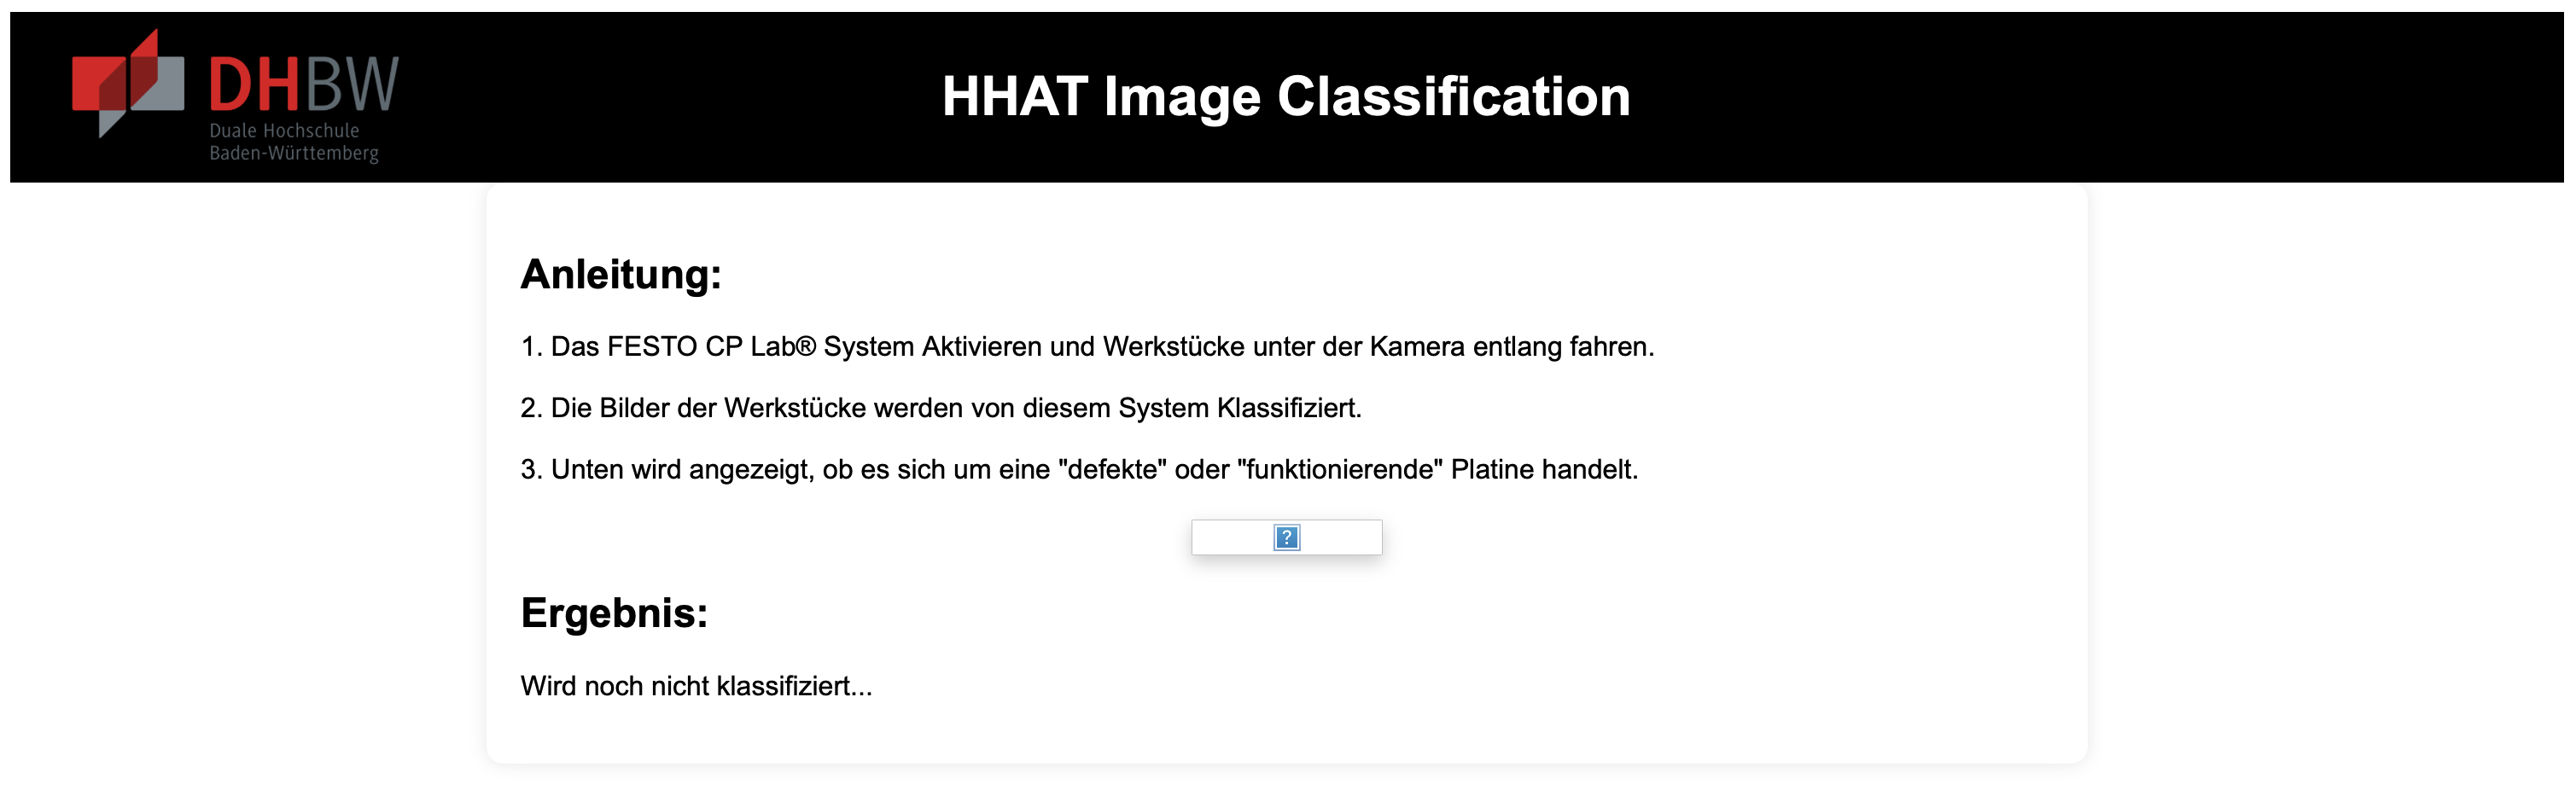
\includegraphics[width=1\textwidth]{Web-Ohne_Bild.png}
    \caption{Darstellung der Weboberfläche im Zustand ohne Klassifikation eines aktuellen Werkstückes.}
    \label{fig:Weboverlay_teststadium}
\end{figure}

Nach der Installation der benötigten Pakete wird die Software getestet. Die Interpretation des übertragenen Python-Codes ist fehlerfrei und der Testbetrieb kann aufgenommen werden. Die finale Gestaltung der Weboberfläche ist in \autoref{fig:Weboverlay_teststadium} dargestellt.

\subsection{Aufgetretene Probleme} \label{subsec:aufgetretene_probleme}

Während der Installation und des Testbetriebs traten zwei Probleme auf, deren Lösung im Folgenden erklärt wird.

Im Testbetrieb fällt auf, dass die Software Bilder nicht korrekt an die Webanwendung übermittelt. Der Grund für das Auftreten dieses Fehlers war ein überschnelles Reagieren des Watchdogs auf neue Bilder. Dieser erkennt eine Datei, bevor sie vollständig in den Ordner übermittelt wurde. Dieses Problem wird durch eine Verzögerung der Bildübermittlung an den Webserver und den Klassifikator behoben. Die Übermittlung startet eine halbe Sekunde nach dem Auslösen des Events.

Der Vision-Sensor, welcher ebenfalls im Lieferumfang des FESTO \ac{cp-lab} Systems enthalten ist, kann mittels der Visor Vision Software verbunden werden \cite{sensopart_industriesensorik_gmbh_visor_2019}. Diese Software ermöglicht eine Anzeige und Konfiguration des Sensors über den Laborrechner. Eine automatisierte Übertragung mittels direkter Verbindung zwischen Laborrechner und Vision-Sensor ist nicht möglich, da dies die Konfiguration des Sensors und damit die Funktionalität des \ac{cp-lab} Systems beeinträchtigen würde.

Um diesen Umstand zu umgehen, wird die Archivierung in der SensoView Software aktiviert. Der hierdurch entstehende Nachteil ist, dass die SensoView Software gestartet und angemeldet sein muss, um die Bilder zu speichern (siehe Anhang \autoref{subsec:anleitung_zur_verwendung}). Zum jetzigen Stand ist eine permanente Lösung ohne Hilfe von FESTO nicht möglich.

\subsection{Neuer Datensatz} \label{subsec:neuer_datzensatz}

Parallel zu dieser Studienarbeit wurde eine weitere Studienarbeit durchgeführt, welche sich mit dem Design neuer \ac{PCB}s beschäftigt. Die detaillierten Änderungen und der Hergang des Designprozesses sind in der Studienarbeit von Herrn Lucas Weyland beschrieben und können dort nachgelesen werden. In dieser Studienarbeit wird diese Änderung als gegeben betrachtet und der neue Datensatz wird für die Klassifikation verwendet. Entsprechend dazu müssen neue Trainingsdaten generiert und das Modell neu trainiert werden.

\begin{figure}[H]
    \centering
    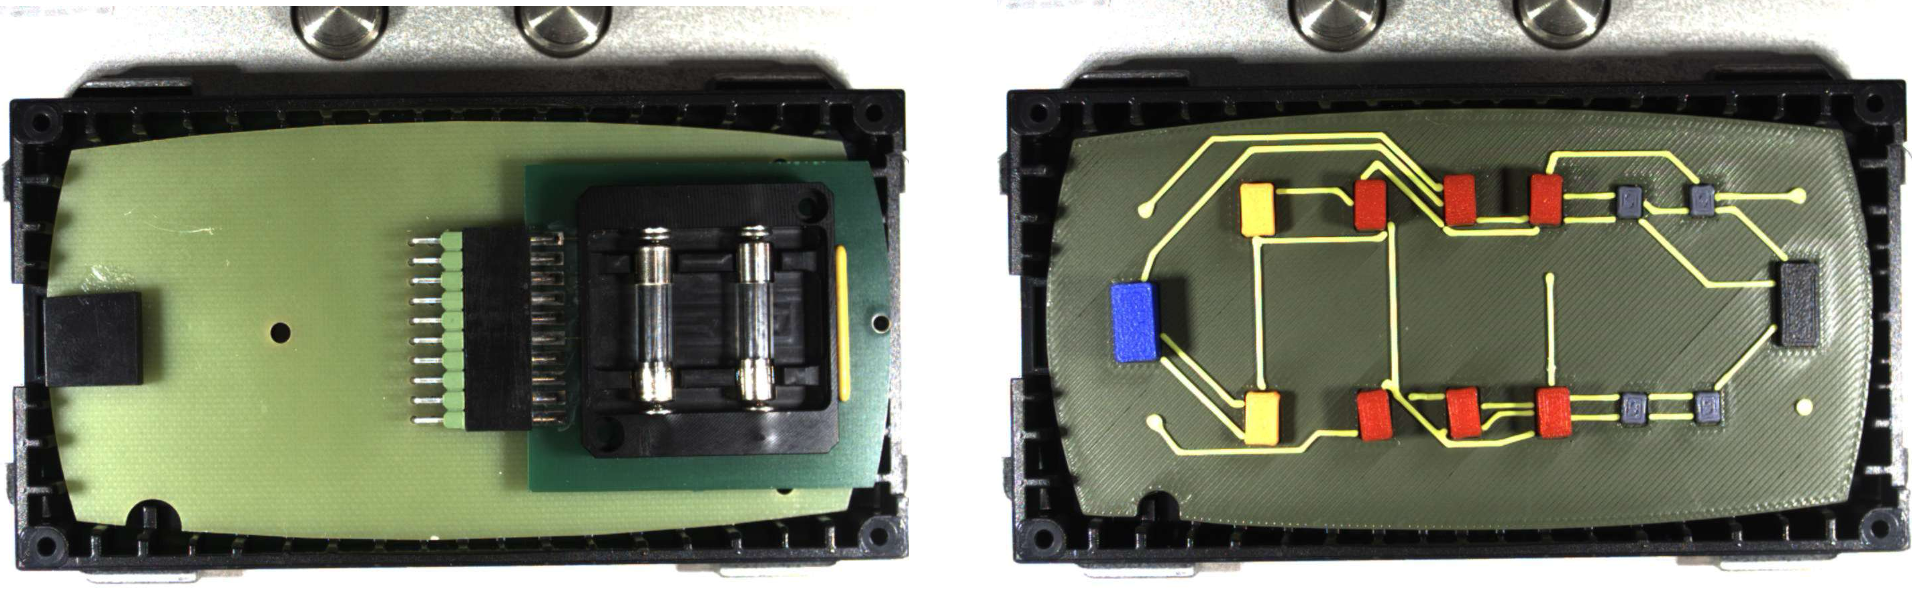
\includegraphics[width=1\textwidth]{PCBs.png}
    \caption{Gegenüberstellung der alten und neuen \ac{PCB}s}
    \label{fig:PCBs}
\end{figure}

Wie auch auf der \autoref{fig:PCBs} zu sehen ist, bieten die neuen PCBs weit mehr Details und sind daher komplexer als die \ac{PCB}s, die für die Machbarkeitsstudie verwendet wurden. 
Dies führt zu mehr Möglichkeiten, die Möglichkeiten des Modells zu testen und die Klassifikation zu verbessern. Die Reevaluierung des Modells mit den neuen Daten wird in \autoref{sec:reevaluierung} beschrieben.


	\chapter{Softwaretests} \label{chap:softwaretests}

In diesem Kapitel wird auf die Evaluierungs- und Testvorgäne für die Sicherstellung der Güte der entwickelten Software eingegangen.
Da es sich bei der entwickelten Software um ein Machine-Learning-Modell handelt, wird in diesem Kapitel auf die Evaluierung des Modells eingegangen. Die Funktionen des interpretierten Python Skripts entwickeln keine neuen Algorithmen, die auf ihre Fehleranfälligkeit oder Korrektheit getestet werden müssen.

\section{Metriken zur Evaluierung} \label{sec:metriken}

Um zu verstehen wie ein Machine Learning Modell evaluiert werden kann ist es zunächst wichtig die Arten von Kriterien nachzuvollzihen, die für die binäre Klassifikation notwendig sind. Im Folgenden wird allgemein von Instanzen gesprochen, es handelt sich dabei um die Bilder, der PCBs die klassifiziert werden sollen.

\begin{itemize}
    \item \textbf{True Positive (TP)}: Die Anzahl der korrekt klassifizierten positiven Instanzen.
    \item \textbf{True Negative (TN)}: Die Anzahl der korrekt klassifizierten negativen Instanzen.
    \item \textbf{False Positive (FP)}: Die Anzahl der falsch klassifizierten positiven Instanzen.
    \item \textbf{False Negative (FN)}: Die Anzahl der falsch klassifizierten negativen Instanzen.
\end{itemize}

Diese wesentlichen Typen teilen die Klassifizierten Daten nach dem Test in vier diskrete Kategorien ein. Diese Kategorien bilden die 
in \autoref{sec:confusionmatrix} beschriebene Confusion Matrix. Mit Ihnen können aber auch die Einfacheren Werte Loss und Accuracy berechnet werden. Im Folgenden wird die Mathematik hinter den Methoden vorgestellt.

\subsection{Accuracy und Loss} \label{sec:accuracy}

Die Accuracy ist eine der einfachsten Metriken zur Evaluierung eines Machine-Learning-Modells. Sie gibt an, wie viele der Instanzen korrekt klassifiziert wurden. Die Accuracy wird vereinfacht wie folgt berechnet:

\begin{equation}
    \text{Accuracy} = \frac{n_{\text{richtig klassifiziert}}}{n_{\text{gesamt}}}
\end{equation}

Bezug auf die in \autoref{sec:metriken} beschriebenen Kategorien, kann die Accuracy wie folgt berechnet werden \cite{ai_wiki_accuracy_2019}:

\begin{equation}
    \text{Accuracy} = \frac{TP + TN}{TP + TN + FP + FN} 
\end{equation}

Die Accuracy wird typischerweise in Prozent angegeben und liegt zwischen 0 und 100\%. Sie ermöglicht eine schnelle Einschätzung der Modellgüte. Allerdings kann die Accuracy irreführend sein, da sie die Anzahl der falsch klassifizierten Instanzen nicht berücksichtigt. Ein Modell, das alle Instanzen als negativ klassifiziert, könnte eine hohe Accuracy aufweisen, obwohl es nicht leistungsfähig ist.

Dennoch ist die Accuracy einfacher zu Interpretieren als der hier vorgestellte Loss. Der Loss ist eine Metrik, die die Güte eines Modells anhand der Wahrscheinlichkeiten der Klassifikationen bewertet. 
Für binäre Klassifikationen wird der Binary Crossentropy Loss verwendet, der wie folgt berechnet wird 
\cite{ai_wiki_accuracy_2019}:

\begin{equation}
    \text{Loss} = -\frac{1}{n} \sum_{i=1}^{n} \left[ y_i \log(\hat{y}_i) + (1 - y_i) \log(1 - \hat{y}_i) \right]
    \label{eq:binary_crossentropy}
\end{equation}

\begin{tabular}{ll}
    \hline
    \textbf{Symbol} & \textbf{Bedeutung} \\
    \hline
    $n$ & Anzahl der Trainingsbeispiele \\
    $k$ & Anzahl der Klassen (bei Mehrklassen-Klassifikation) \\
    $y_i$ & Wahre Klasse (0 oder 1) für das $i$-te Beispiel \\
    $\hat{y}_i$ & Vorhergesagte Wahrscheinlichkeit für Klasse 1 \\
    \hline
\end{tabular}

In jeder Epoche des Trainings werden beide Werte berechnet und stellen so die Verbesserung des Modells dar. Der Loss wird dabei minimiert, während die Accuracy maximiert wird. Bereits in der Letzten Studienarbeit wurden die geteste Modelle anhand dieser Metriken evaluiert.

\subsection{Confusion Matrix und F1 Score} \label{sec:confusionmatrix}

Eine aussagekräftigere Methode zur Evaluierung ist der F1 Score. Um diesen nachzuvollziehen ist zunächst eine aufschlüsselung der Klassifizierten Daten notwendig. Die Confusion Matrix ist eine Tabelle, die die Anzahl der korrekten und falschen Klassifikationen für jede Klasse anzeigt. Die Confusion Matrix hat die folgende Form \cite{lipton_thresholding_2014}:

\[
\begin{array}{c|cc}
    & \textbf{Vorhergesagt: Positiv} & \textbf{Vorhergesagt: Negativ} \\
    \hline
    \textbf{Tatsächlich Positiv} & TP & FN \\
    \textbf{Tatsächlich Negativ} & FP & TN
\end{array}
\]

Hier sind die Werte TP, FP, TN und FN die in \autoref{sec:metriken} bereits eingeführt wurden wieder zu finden. Auf der Hauptdiagonale dieser $2x2$ Matrix befinden sich die korrekt klassifizierten Instanzen, während auf der nebendiagonale die falsch klassifizierten Instanzen zu finden sind. 

Für jeden Evaluierungsaufruf lässt sich diese Matrix bestimmen. Vorteilhaft an dieser Darstellung ist, dass die Möglichtkeit besteht dieses Modell auf nicht binäre Klassifikation zu erweitern. 

Aus dieser Matrix lassen sich nun weitere Metriken ableiten. Eine davon ist der F1 Score. Der F1 Score ist das harmonische Mittel zwischen Precision und Recall. Precision gibt an, wie viele der als positiv klassifizierten Instanzen tatsächlich positiv sind, während Recall angibt, wie viele der tatsächlich positiven Instanzen korrekt klassifiziert wurden. Der F1 Score wird wie folgt berechnet \cite{lipton_thresholding_2014}:

\begin{equation}
    \text{F1} = \frac{2 TP}{2 TP + FP + FN }
\end{equation}

Beispielhafte Confusion Matritzen werden in \autoref{sec:reevaluierung} vorgestellt.

\section{Reevaluierung des Modells} \label{sec:reevaluierung}

In diesem Kapitel soll das Ergebnismodell der letzten Studienarbeit, \texttt{"Mobilenet"} erneut Evaluiert werden. Diesmal mithilfe der neuen Metrinken (\autoref{sec:confusionmatrix})

Da es sich bei Mobilnet und XX um vortrainierte Modelle von Tensorflow sind, soll auch ein selbstgeschriebenes Modell evaluiert werden. Dieses Modell \texttt{"Pytorchmodel"} wurde im Rahmen der Vorlesung Bildverarbeitung entwickelt und soll nun mit in die Tests einfließen. 

\begin{figure}[h]
    \centering
    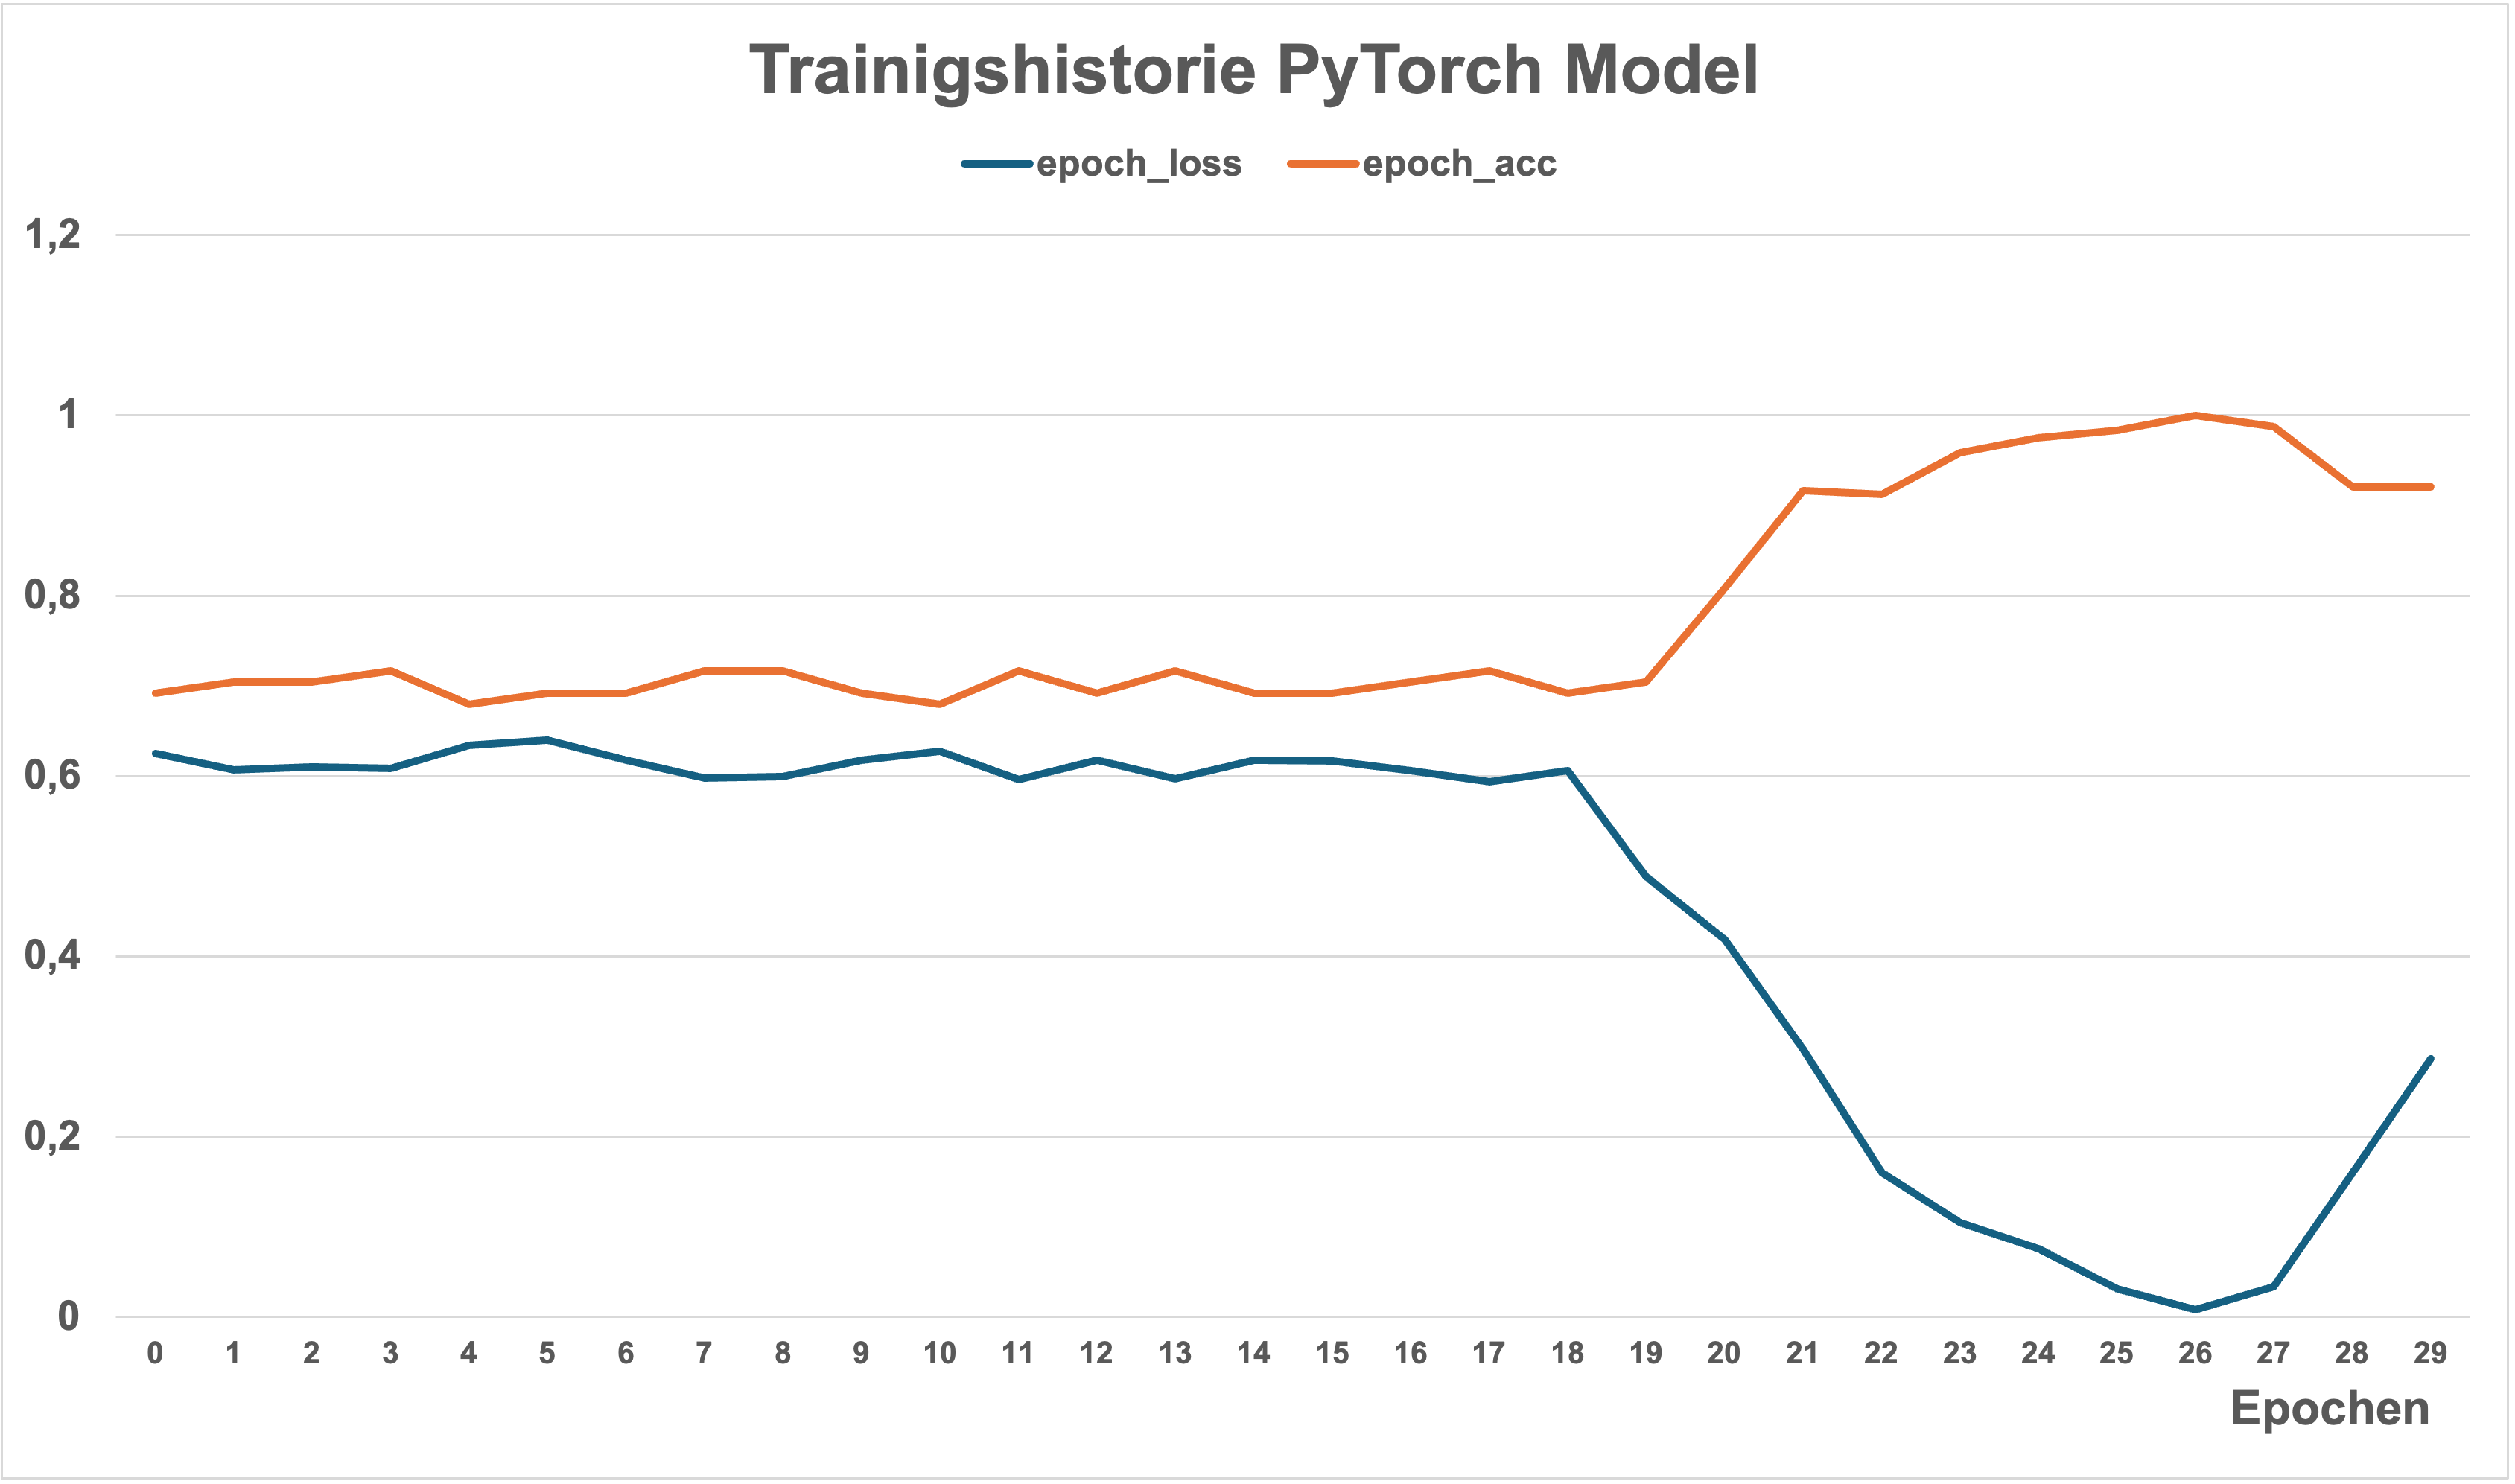
\includegraphics[width=1\textwidth]{Training_PyTorch.png}
    \caption{Schematischer Aufbau der API Kommunikation}
    \label{fig:Training_PyTorch}
\end{figure}
	
\chapter{Fazit und Ausblick} \label{chap:fazit_und_ausblick}

In dieser Arbeit wurde ein bestehendes Projekt zur Bildklassifikation von Leiterplattenfehlern weiterentwickelt und evaluiert. Der Schwerpunkt lag dabei auf der Implementierung einer Schnittstelle zur besseren Verwendbarkeit und Präsentierparkeit des bestehenden Projekts. Darüber hinaus wurden verschiedene Modelle und Methoden zur Bildklassifikation anhand eines neuen Datensatzes untersucht und miteinander verglichen.

Trotz der erzielten Fortschritte gibt es mehrere Bereiche, die für zukünftige Arbeiten von Interesse sein könnten. Eine mögliche Erweiterung besteht darin, die Integration des Custom CNN in die Programmpipeline zu ermöglichen. Darüber hinaus könnten weitere Modelle und Methoden zur Bildklassifikation untersucht und verglichen werden, um die bestmögliche Leistung zu erzielen.

Ergebnis ist eine Funktionierende Webanwendung, die es ermöglicht, neue Bilder des FESTO \ac{cp-lab} darzustellen, zu klassifizieren und die Ergebnisse auf einer Weboberfläche zu visualisieren. Die Anwendung koordiniert die Überwachung eines Ordners für neue Bilder und die Klassifizierung dieser Bilder in defekt oder nicht defekt. Die Implementierung erfolgte in Python unter Verwendung der Flask-Bibliothek für die Webanwendung und der TensorFlow-Bibliothek für die Bildklassifikation. Der Quellcode für dieses Projekt ist auf GitHub verfügbar und kann von Interessierten eingesehen und weiterentwickelt werden. Der Link zu diesem Repository und einer Anleitung ist im Anhang \autoref{subsec:anleitung_zur_verwendung} zu finden.

Eine weitere mögliche Fortsetzung dieser Studienarbeit wäre die Implementierung von Ensemble Methoden, bei denen mehrere Modelle kombiniert werden, um die Klassifikationsergebnisse zu verbessern. Dies könnte insbesondere bei komplexen Datensätzen von Vorteil sein, bei denen einzelne Modelle möglicherweise nicht die bestmögliche Leistung erzielen.

Zukünftige Arbeiten sollten sich darauf konzentrieren, die Integration des Custom CNN in die Programmpipeline zu ermöglichen, um die Leistung der Klassifikation weiter zu verbessern.
	
	
	\cleardoublepage % sicherstellen, dass das Literaturverzeichnis auf einer neuen Seite beginnt
	\pagenumbering{Roman}
	
	% Fortsetzung der Nummerierung: Stelle sicher, dass die Nummerierung weitergeht
	\setcounter{page}{10}
	% Literaturverzeichnis
	\addcontentsline{toc}{chapter}{Literaturverzeichnis}\printbibliography[title=Literaturverzeichnis]
	
	\appendix
\renewcommand{\thesection}{\Alph{section}} % Nummerierung mit Buchstaben
\renewcommand{\thesubsection}{\thesection.\arabic{subsection}} % Zweite Ebene mit Zahlen
\renewcommand*{\sectionmark}[1]{\markright{Anhang \thesection: #1}}

\chapter{Anhang}
	

	
\end{document}
